\subsection{Class diagram di analisi o dominio}

    \begin{flushleft}
        Class diagram di analisi servono a bla bla bla\ldots
        Some description over here\ldots
    \end{flushleft}

    \subsubsection{Class diagram Login}
        \begin{figure}[H]
            \centering
            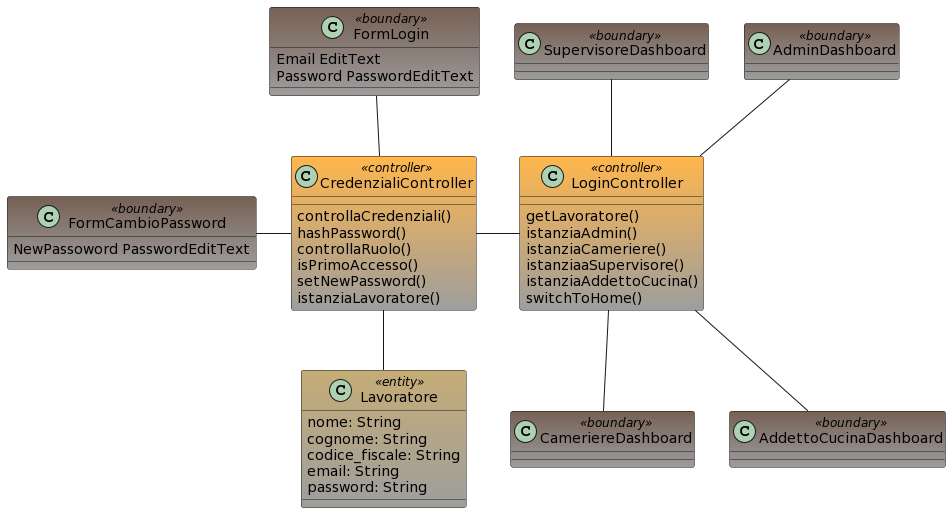
\includegraphics[scale=0.5]{assets/diagrammi/Class diagram di analisi/Login_3.png}
            \caption{\textbf{C01}: Class diagram Login}\label{fig:Login}
        \end{figure}

    \subsubsection{Class diagram Ristorante}
        \begin{figure}[H]
            \centering
            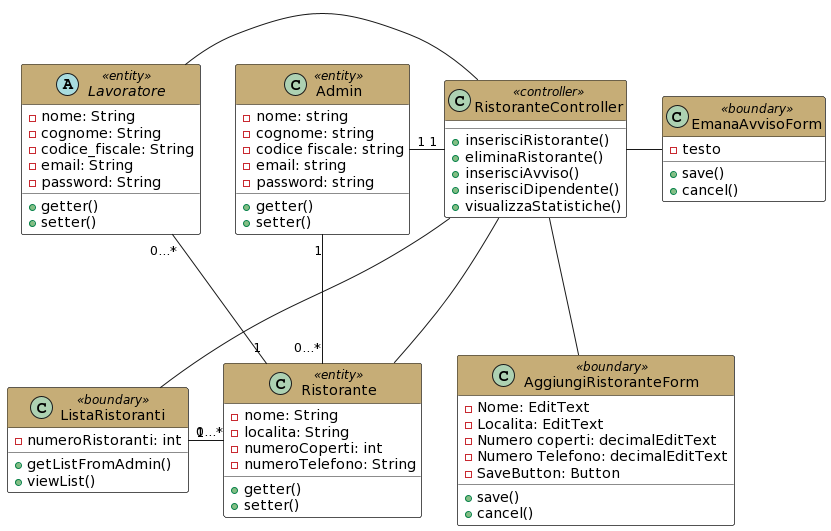
\includegraphics[scale=0.5]{assets/diagrammi/Class diagram di analisi/Gestione ristorante.png}
            \caption{\textbf{C02}: Class diagram Gestione ristorante}\label{fig:Ristorante}
        \end{figure}

    \subsubsection{Class diagram dipendenti}
        \begin{figure}[H]
            \centering
            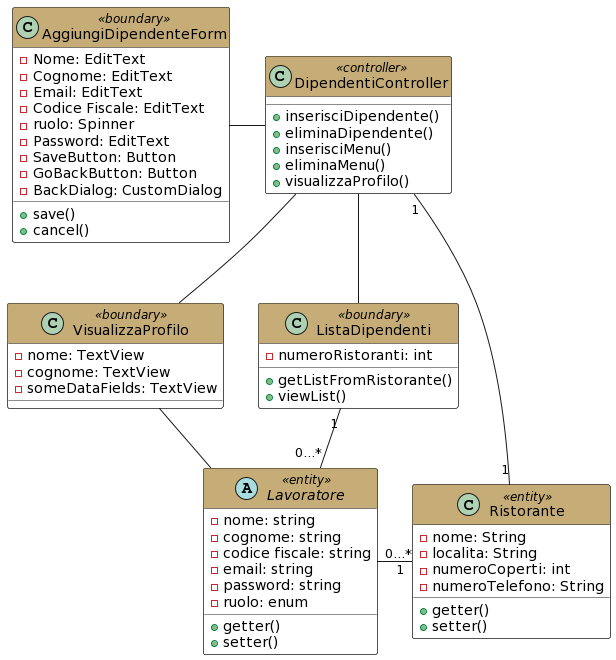
\includegraphics[scale=0.5]{assets/diagrammi/Class diagram di analisi/Gestione dipendenti.png}
            \caption{\textbf{C03}: Class diagram gestione dipendenti}\label{fig:Dipendenti}
        \end{figure}
    
    \subsubsection{Class diagram Menu}
        \begin{figure}[H]
            \centering
            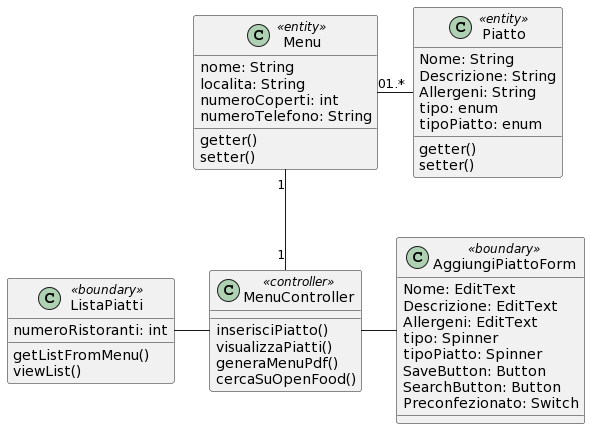
\includegraphics[scale=0.5]{assets/diagrammi/Class diagram di analisi/Gestione menu.png}
            \caption{\textbf{C04}: Class diagram gestione menu}\label{fig:Menu}
        \end{figure} 

    \subsubsection{Class diagram Avvisi}
        \begin{figure}[H]
            \centering
            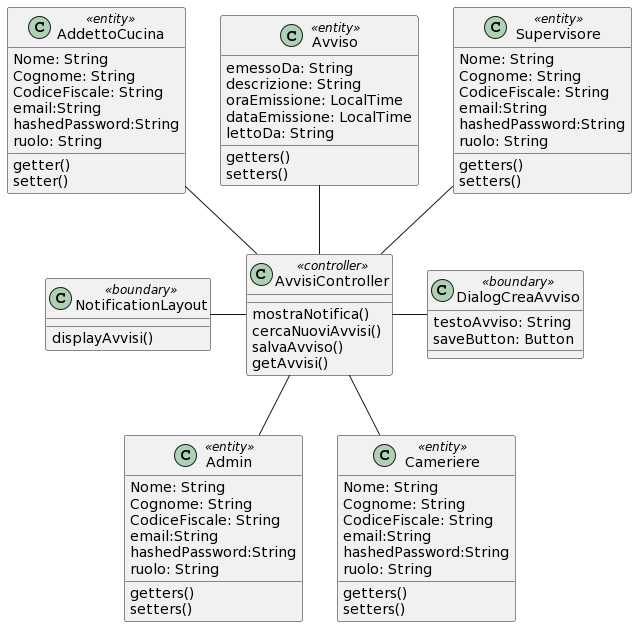
\includegraphics[scale=0.5]{assets/diagrammi/Class diagram di analisi/Gestione Avvisi.png}
            \caption{\textbf{C05}: Class diagram gestione avvisi}\label{fig:Avvisi}
        \end{figure}

    \subsubsection{Class diagram Ordini}
        \begin{figure}[H]
            \centering
            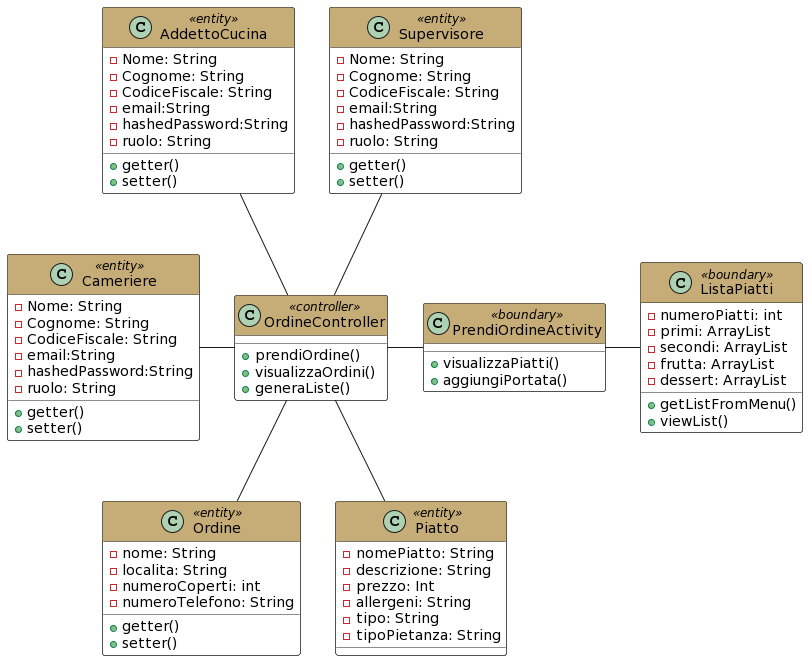
\includegraphics[scale=0.5]{assets/diagrammi/Class diagram di analisi/Gestione ordini.png}
            \caption{\textbf{C06}: Class diagram gestione ordini}\label{fig:Ordini}
        \end{figure}

    \subsubsection{Class diagram statistiche}
        \begin{figure}[H]
            \centering
            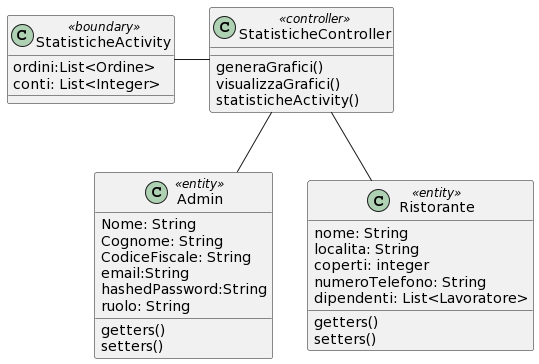
\includegraphics[scale=0.5]{assets/diagrammi/Class diagram di analisi/Gestione Stat.png}
            \caption{\textbf{C07}: Class diaram gestione statistiche}\label{fig:Statistiche}
        \end{figure}